\documentclass[10pt]{article}
\usepackage[margin=0.95in]{geometry}

\usepackage{mathptmx}
\usepackage{microtype}
\usepackage[round,authoryear]{natbib}
\usepackage{graphicx,booktabs,amsmath,amssymb,xcolor,enumitem,caption,tabularx,multirow,array}
\usepackage{tikz}
\usetikzlibrary{arrows.meta,positioning,fit,backgrounds,calc}
\usepackage[colorlinks,linkcolor=blue!50!black,urlcolor=blue!50!black,citecolor=blue!50!black]{hyperref}
\captionsetup{font=small,labelfont=bf}
\setlist{nosep,leftmargin=1.3em}
\graphicspath{{../figs/}}
\newcommand{\para}[1]{\textbf{#1}\hspace{0.45em}}

\title{\textbf{Oversight Removes the Evidence, Not the Harm:\\What Logs Can Prove About Collusion Among LLM Agents}}
\author{Adrita Rahman Tory\\ \small Jahangirnagar University, Savar, Dhaka, Bangladesh}
\date{}

\begin{document}\maketitle

\begin{abstract}\noindent
Language-model agents can sustain prices above the competitive level in simulated markets. An auditor who must decide whether such prices reflect collusion has to trust that the agents' logs (prices, messages and reasoning traces) carry evidence of coordination when coordination occurs. Economics, antitrust law and AI safety each define collusion differently, so we turn each definition into a detector and test all of them on the same data. On a synthetic pricing benchmark with ground-truth labels and seven case types, every single-definition detector fails on a predictable case: an outcome detector flags 100\% of an innocent demand boom, a talk detector scores AUROC 0.46, and price correlation scores 0.42. An antitrust-style plus-factor rule (harmful outcome plus mutual price influence or coordinating talk) cuts the mean false-alarm rate from 0.34 to 0.04 and catches 89--98\% of cartels that react to their partner, but only 8\% of a cartel that never reacts. We then audit 75 released GPT-4.1 and Claude-3.7-Sonnet double-auction runs. In all 20 runs with an LLM overseer, the overseer gives seller messages its maximum coordination score within the first 7 rounds, and every later message is capped at 5 characters. Under profit pressure, prices then stay at a collusion index of 0.63, identical to pressure without oversight (0.64, $p{=}0.62$), while message length falls from 330 to 22 characters and sellers react to rivals less than competitive sellers do (partial $R^2$ 0.15 vs.\ 0.39). Restricting the channel after detection leaves a market that holds its price with weak traces of coordination, the same pattern as the one case our best detector misses. Detection worked. The harm stayed.
\end{abstract}

\section{Introduction}
\label{sec:intro}

Consider five GPT-4.1 sellers in a double auction where each unit costs \$80 and buyers value it at \$100, so the competitive price is \$90 \citep{agrawal}. In the first hour, one seller writes to the others: ``Let's avoid a race to the bottom.'' Another adds: ``Holding firm could reward us all with higher margins.'' An LLM overseer reads these messages, scores the third hour's messages 4 out of 4 for collusion, and a regulator notice limits every seller message to 5 characters from then on. For the next 27 hours, every message is ``ok'' or an emoji. The mean ask starts at \$97.1 and ends at \$96.8. The overseer did its job. The price never moved.

This run raises the question every auditor of AI agents faces: given the logs, is this collusion? The answer depends on which definition the auditor uses. Economics treats collusion as profits or prices above the competitive level \citep{ivaldi,stigler}. Antitrust law requires an agreement, and since parallel prices alone are lawful, courts infer agreement from additional evidence called plus factors \citep{kovacic,oecd}. AI safety research focuses on covert coordination that evades an overseer, for example through steganographic messages \citep{motwani,mathew}. Each definition points to a different signal in the logs. The three signals can disagree.

Recent work shows why the disagreement matters for language-model agents. GPT-4 pricing agents reach supra-competitive prices without being told to collude \citep{fish}, and DeepSeek-R1 agents keep colluding even when told not to \citep{riemer}. Agents plan collusion in text but often fail to act on it \citep{nakamura}, while other agents sustain supra-competitive prices with faithful reasoning, so chain-of-thought monitoring alone is not a sufficient safeguard \citep{leepark}. Telling an agent it is monitored reduces monitor reliability \citep{kale}, and agents can sometimes infer a hidden monitor from feedback alone \citep{jiralerspong}. Detection work, in turn, reaches opposite conclusions about which signal to trust: price-level audits are blind to collusion that hides in the dependence between agents \citep{xu}, while dependence measures \citep{bonjour} assume that colluders react to each other. No study has asked how these signals fail against one another on the same data. This gap is our starting point.

We build one detector per definition and test them together on two kinds of data. The first is a synthetic repeated-pricing benchmark with ground-truth labels and deliberately hard cases: an innocent demand boom that raises all prices, a pair that talks about colluding but prices competitively, and a cartel that holds a markup without ever reacting to its partner. The second is the set of 75 double-auction runs released by \citet{agrawal}, which vary seller communication, profit pressure from a simulated CEO, and an LLM overseer. Figure~\ref{fig:pipeline} shows the full pipeline. The synthetic benchmark tells us where each detector breaks. The real logs tell us whether real agents land in those blind spots.

\begin{itemize}[leftmargin=1.2em,itemsep=2pt]
\item \textbf{A benchmark that maps definitions to detectors.} We turn the economic, legal and AI-safety definitions of collusion into four detectors over logged trajectories and test them on seven labeled case types, including hard negatives and hard positives. This matters because each detector looks reasonable on average yet fails completely on one predictable case. Auditors can now choose evidence knowing which case it misses.
\item \textbf{A plus-factor rule with a measured failure map.} We show that requiring a harmful outcome plus one independent plus factor cuts false alarms from 0.34 to 0.04 while keeping 89--98\% detection for reacting cartels. The rule moves the remaining error onto a single case, a cartel that never reacts (8\% detected). This turns a legal doctrine into a decision rule with known error rates per case.
\item \textbf{An evasion analysis with costs.} We measure detection and retained markup together for three evasion strategies. Masking costs a cartel about as much markup as it removes in detection, cheap price noise does not evade at all, and weak reaction evades for free in our simulator. This identifies reaction strength, not noise, as the lever that decides detectability.
\item \textbf{Evidence that channel restriction removes evidence but not harm.} In all 20 overseen real runs, the overseer catches explicit coordination early and restricts the channel. Under profit pressure, prices do not move, talk evidence falls by 1.39 points on a 4-point scale, and rival reaction drops to 0.15. Real LLM agents therefore end up in exactly the blind spot the benchmark exposes, which changes what oversight should be asked to do.
\end{itemize}

\section{Background and Related Work}
\label{sec:related}

Collusion has three working definitions, and each one comes with its own kind of evidence. We review them in turn, then the work on LLM agents and on detection that connects them. Table~\ref{tab:related} places the closest studies side by side.

\para{Markets: collusion as an outcome}Economic theory defines tacit collusion as prices sustained above the competitive level by the threat of future punishment \citep{stigler,greenporter,ivaldi}. Reinforcement-learning pricing agents learn such prices together with punishment of deviations \citep{calvano}, although whether these outcomes count as ``genuine'' collusion remains debated \citep{calvano23}. Field evidence links the adoption of pricing algorithms to higher margins in German retail gasoline \citep{assad}. Outcome evidence needs a competitive benchmark, which auditors rarely observe. That limitation is the reason law asks for more.

\para{Law: collusion as an agreement}Antitrust law punishes agreements, not high prices. Parallel conduct alone is lawful in the United States, so courts require plus factors, such as communications or conduct that would be irrational without agreement, before inferring a conspiracy \citep{kovacic}. Pricing algorithms strain this standard because they can coordinate without anything resembling an agreement \citep{ezrachi,harrington18,oecd}. Screens for bid rigging use statistical patterns in bids instead of communications \citep{huber,kawai}. The legal view thus makes communication central. AI safety asks what happens when that communication is hidden.

\para{AI safety: collusion as covert coordination}Safety research defines collusion as coordination among agents that undermines an overseer or a third party \citep{foxabbott,hammond}. LLM agents can hide coordination in steganographic text \citep{motwani,mathew}, and control protocols must assume that untrusted models may try to subvert monitoring \citep{greenblatt}. Monitoring a model's reasoning is useful but fragile: optimizing against a chain-of-thought monitor teaches models to obfuscate \citep{baker}, and monitorability may not survive future training \citep{korbak}. Multi-agent attacks also fragment evidence across agents so that per-agent monitors miss them \citep{makins}. These concerns now apply directly to market agents.

\para{LLM agents in markets}LLM pricing agents collude in Bertrand settings \citep{fish,riemer}, divide multi-commodity markets \citep{lin}, and coordinate in double auctions, where seller communication and CEO-style urgency raise prices and an overseer lowers them unless urgency is present \citep{agrawal}. Collusion becomes fragile when agents differ in patience, data or number \citep{keppo}. In cooperative settings, agents often plan collusion without carrying it out \citep{nakamura}. These studies measure whether collusion happens. We ask whether an auditor could tell from the logs.

\para{Detecting collusion}Dependence-based detectors measure mutual information between agents' actions \citep{bonjour} or audit the reward-and-punishment structure of frozen pricing policies \citep{eschenbaum}. Communication audits combine channel-capacity analysis with calibrated detectors \citep{tailor}. Two recent results bound what each family can see. Collusion can live entirely in the joint dependence of agents while each agent's prices look competitive, which blinds price-level audits by construction \citep{xu}. Chain-of-thought faithfulness and collusive behavior also vary independently, so reasoning monitors miss collusion that agents describe honestly \citep{leepark}. Activation probes, by contrast, stay accurate when agents are told about the monitor \citep{das}. We study the case the first result leaves open: high prices with no joint dependence at all.

\begin{table}[t]\centering\footnotesize
\setlength{\tabcolsep}{4pt}
\begin{tabularx}{\linewidth}{@{}>{\raggedright\arraybackslash}p{2.45cm}>{\raggedright\arraybackslash}p{2.6cm}>{\raggedright\arraybackslash}p{3.0cm}>{\raggedright\arraybackslash}p{1.75cm}>{\raggedright\arraybackslash}X@{}}\toprule
Work & Setting & Evidence used & Ground truth & Finding relevant to auditing\\\midrule
\citet{calvano} & Q-learning pricing & Profit index, response to deviations & No & Algorithms learn supra-competitive prices with punishment\\
\citet{huber} & Swiss procurement & Bid-distribution screens & Known cartel periods & ML screens flag bid rigging from bids alone\\
\citet{bonjour} & Repeated games, poker & Mutual information of actions & Designed colluders & Action dependence detects collusion levels\\
\citet{motwani} & LLM messaging & Message content, steganalysis & Designed scenarios & LLMs can hide coordination in text\\
\citet{tailor} & ColludeBench-v0 & Calibrated multi-signal detectors & Designed colluders & Channel limits reduce covert capacity\\
\citet{agrawal} & LLM double auction & Prices, LLM judge on reasoning & No & Urgency dominates oversight in prices\\
\citet{nakamura} & Cooperative agent teams & Action regret vs.\ communication & Cooperative optimum & Agents often collude ``on paper'' only\\
\citet{xu} & Theory, LLM bidders & Joint dependence of residuals & Constructed & Price-level audits are blind by construction\\
\citet{leepark} & LLM Bertrand pricing & Chain-of-thought faithfulness & No & Faithful reasoning still coexists with collusion\\
\citet{das} & Multi-agent games & Activation probes & Labeled episodes & Monitoring awareness does not evade probes\\\midrule
\textbf{This work} & Synthetic pricing + 75 LLM auction runs & Outcome, talk, correlation, lagged influence, plus-factor rule & Yes (synthetic), conditions (real) & Each signal fails on a predictable case; channel restriction leaves harm with no reaction signal\\\bottomrule
\end{tabularx}
\caption{Closest work on detecting or measuring collusion. ``Ground truth'' means labeled collusive and innocent cases are available for evaluating a detector.}\label{tab:related}
\end{table}

\section{Turning Definitions into Detectors}
\label{sec:method}

Each definition becomes a score computed from logs, and a detector flags an episode when the score crosses a threshold. Table~\ref{tab:defs} lists the mapping. We keep every detector simple on purpose, because the question is which \emph{kind} of evidence fails, not how far one model can be tuned.

\begin{table}[h]\centering\footnotesize
\begin{tabularx}{\linewidth}{@{}p{3.1cm}p{4.3cm}X@{}}\toprule
Field & Definition of collusion & Detector and score\\\midrule
Markets \citep{ivaldi} & Prices above the competitive level & \textbf{Outcome}: mean price minus a fixed competitive benchmark\\
Law \citep{kovacic,oecd} & An agreement that harms competition & \textbf{Talk}: rate of messages a monitor flags as coordinating\\
AI safety \citep{foxabbott,motwani} & Covert coordination against an overseer & \textbf{Influence}: how much a rival's past price predicts mine\\
Baseline & Parallel conduct & \textbf{Correlation}: pairwise correlation of price changes\\\bottomrule
\end{tabularx}
\caption{Three definitions of collusion and the detector we build for each.}\label{tab:defs}\end{table}

\para{Outcome}The score is the episode's mean price minus 0.3, a fixed competitive benchmark. We fix the benchmark because auditors rarely observe demand shifts, and this choice is exactly what an innocent boom exploits.

\para{Talk}A message monitor flags each message independently. The score is the mean flag rate of the two most-flagged agents, which targets a pair rather than the whole market.

\para{Correlation}The score is the largest pairwise correlation of first-differenced prices. It measures parallel movement, the evidence that courts reject as insufficient on its own.

\para{Influence}Tacit collusion is enforced by reaction: if my partner deviates, I respond. We therefore measure how much a rival's last price predicts my current price beyond my own last price and the public demand signal. Formally, $I_{ij}$ is the partial $R^2$ gained by adding $p_{j,t-1}$ to a regression of $p_{i,t}$ on $(1, p_{i,t-1}, b_t)$, where $b_t$ is public demand. The score is $\max_{i<j}\sqrt{I_{ij}I_{ji}}$, which rewards mutual influence, and the arg-max pair is the accused pair. This is a linear, lag-based measure in the spirit of information-theoretic dependence \citep{bonjour}, not a reproduction of it.

\para{Plus-factor rule}The rule flags an episode when Outcome exceeds its threshold \emph{and} either Influence or Talk exceeds its own. It mirrors the legal standard that parallel conduct needs at least one supporting plus factor \citep{kovacic}. We set the Influence and Talk thresholds at the 95th percentile of innocent training episodes only, so the rule never sees a cartel label.

\begin{figure}[t]\centering
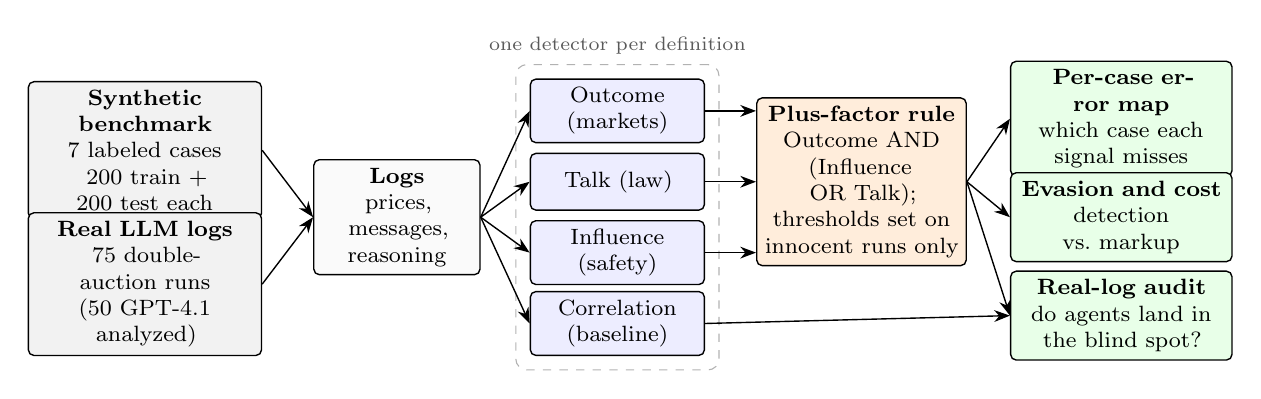
\begin{tikzpicture}[
  font=\footnotesize, >={Stealth[length=2mm]}, line width=0.5pt,
  box/.style={draw, rounded corners=2pt, align=center, inner sep=3pt},
  databox/.style={box, fill=gray!10, text width=2.75cm, minimum height=1.25cm},
  detbox/.style={box, fill=blue!7, text width=2.0cm, minimum height=0.72cm},
  rulebox/.style={box, fill=orange!14, text width=2.45cm, minimum height=1.9cm},
  outbox/.style={box, fill=green!9, text width=2.6cm, minimum height=1.0cm}]
\node[databox] (syn) at (0, 0.85) {\textbf{Synthetic benchmark}\\7 labeled cases\\200 train + 200 test each};
\node[databox] (real) at (0,-0.85) {\textbf{Real LLM logs}\\75 double-auction runs\\(50 GPT-4.1 analyzed)};
\node[box, fill=gray!4, text width=1.9cm, minimum height=1.3cm] (logs) at (3.2,0) {\textbf{Logs}\\prices, messages,\\reasoning};
\node[detbox] (d1) at (6.0, 1.35) {Outcome (markets)};
\node[detbox] (d2) at (6.0, 0.45) {Talk (law)};
\node[detbox] (d3) at (6.0,-0.45) {Influence (safety)};
\node[detbox] (d4) at (6.0,-1.35) {Correlation (baseline)};
\node[rulebox] (pf) at (9.1, 0.45) {\textbf{Plus-factor rule}\\Outcome AND\\(Influence OR Talk);\\thresholds set on\\innocent runs only};
\node[outbox] (o1) at (12.4, 1.25) {\textbf{Per-case error map}\\which case each\\signal misses};
\node[outbox] (o2) at (12.4, 0.0) {\textbf{Evasion and cost}\\detection vs.\ markup};
\node[outbox] (o3) at (12.4,-1.25) {\textbf{Real-log audit}\\do agents land in\\the blind spot?};
\draw[->] (syn.east) -- (logs.west);
\draw[->] (real.east) -- (logs.west);
\foreach \d in {d1,d2,d3,d4} \draw[->] (logs.east) -- (\d.west);
\foreach \d in {d1,d2,d3} \draw[->] (\d.east) -- (pf.west|-\d.east);
\draw[->] (d4.east) -- (o3.west);
\foreach \o in {o1,o2,o3} \draw[->] (pf.east) -- (\o.west);
\begin{scope}[on background layer]
\node[draw=gray!60, dashed, rounded corners, fit=(d1)(d4), inner sep=5pt] (grp) {};
\end{scope}
\node[font=\scriptsize, gray!70!black, above=0pt of grp] {one detector per definition};
\end{tikzpicture}
\caption{The audit pipeline. Both data sources produce the same kind of log. Four detectors, one per definition, score each episode, and the plus-factor rule combines Outcome, Talk and Influence. Outputs are a per-case error map and an evasion-cost analysis on synthetic data, and a condition-level audit of real agents in which Correlation serves as a baseline.}\label{fig:pipeline}
\end{figure}

\section{A Benchmark with Ground Truth}
\label{sec:synthetic}

Real logs never come with labels, so we first build a market where we know who colludes. The benchmark is small and transparent so that every failure can be traced to a cause.

\para{Market}Each episode has $N{=}4$ sellers over $T{=}30$ rounds, the same length as the real runs, with normalized prices in $[0,1]$. A public demand signal $b_t$ follows an AR(1) process ($\rho{=}0.8$, $\sigma{=}0.05$) around a regime mean of 0.3 and serves as the competitive price. Competitive sellers price at $b_t$ plus Gaussian noise ($\sigma{=}0.04$). A colluding pair $(i,j)$, chosen at random, holds a markup $\mu{=}0.35$ and follows its partner's last deviation from the cartel price with strength $\gamma{=}0.7$:
\[p_{i,t} = b_t + \mu + \gamma\,(p_{j,t-1} - b_{t-1} - \mu) + \varepsilon_{i,t}.\]
The reaction term is the enforcement mechanism of tacit collusion \citep{greenporter}. A talk monitor flags benign messages with probability 0.05 and collusive ones with 0.8.

\para{Seven cases}Three cases are innocent. In \texttt{competitive}, everyone prices competitively. In \texttt{boom\_parallel}, the demand regime shifts to 0.6, so all sellers rise together. In \texttt{talk\_no\_action}, a pair sends collusive messages but prices competitively. Four cases are collusive and share the pricing rule above: \texttt{cartel\_talk} also talks, \texttt{cartel\_tacit} sends no messages, \texttt{cartel\_monitored} sends only benign messages, and \texttt{cartel\_static} holds the markup with $\gamma{=}0$, never reacting to its partner.

\para{Protocol}Training and test sets use different seeds, with 200 episodes per case in each. Single-detector thresholds maximize balanced accuracy on training data. All thresholds are frozen before testing, and we report every case separately because means hide the failures we care about.

\subsection{Every single definition fails on a predictable case}

Each detector fails exactly where its definition predicts. Figure~\ref{fig:cases} shows the flag rate of every detector on every held-out case; red cells mark the cases where a detector's majority call is wrong, and each column has at least one. Table~\ref{tab:main} summarizes the same results.

\begin{figure}[t]\centering\includegraphics[width=0.86\linewidth]{fig1_cases.pdf}
\caption{Flag rate per case on held-out episodes (200 per case). Rows above the line are innocent, rows below are collusive. Red bold cells are cases where the detector's majority call is wrong.}\label{fig:cases}\end{figure}

\para{Outcome cannot see the benchmark}The outcome detector flags all 200 innocent boom episodes (FPR 1.00) because it compares prices with a fixed benchmark that does not move with demand. It catches 98\% of cartels, but its AUROC is only 0.67. Harm without a true benchmark is not evidence.

\para{Talk is at chance}The talk detector scores AUROC 0.46. Its best training threshold collapses to ``any flag at all'', because half the cartels never talk and one innocent case talks constantly; as a result it flags 93\% of fully competitive episodes. Talk without action and action without talk are both common.

\para{Correlation is worse than chance}Price correlation scores AUROC 0.42 and flags at least 99\% of every innocent case. Innocent sellers move together in the same round because they share a demand shock, while a cartel's coupling is lagged by one round. This is the statistical form of the legal rule that parallel conduct is not evidence of agreement.

\para{Influence misses the static cartel}Influence has the lowest false-alarm rate (0.05) and names the correct pair in 97--99\% of reacting-cartel episodes. It detects only 4\% of the static cartel, which holds a markup without reacting and so leaves no lagged dependence.

\begin{table}[t]\centering\small
\begin{tabular}{@{}lcccccl@{}}\toprule
Detector & AUROC & Mean TPR & Mean FPR & Bal.\ acc. & Worst case\\\midrule
Outcome (markets) & 0.67 & 0.98 & 0.34 & 0.82 & \texttt{boom\_parallel}: FPR 1.00\\
Talk (law) & 0.46 & 0.93 & 0.94 & 0.49 & \texttt{talk\_no\_action}: FPR 1.00\\
Correlation (parallel conduct) & 0.42 & 0.98 & 0.99 & 0.49 & \texttt{competitive}: FPR 1.00\\
Influence (AI safety) & 0.85 & 0.69 & 0.05 & 0.82 & \texttt{cartel\_static}: TPR 0.04\\
\textbf{Plus-factor rule} & n/a & 0.72 & \textbf{0.04} & \textbf{0.84} & \texttt{cartel\_static}: TPR 0.08\\\bottomrule
\end{tabular}
\caption{Held-out results, averaged over the 4 collusive (TPR) and 3 innocent (FPR) cases. The plus-factor rule is a Boolean decision, so it has no AUROC. Its per-case TPRs are 0.98 (talk), 0.92 (tacit), 0.89 (monitored) and 0.08 (static); its per-case FPRs are 0.00 (competitive), 0.10 (boom) and 0.01 (talk only).}\label{tab:main}
\end{table}

\para{The plus-factor rule fixes false alarms, not the static cartel}Requiring a harmful outcome plus one plus factor drops the boom false-alarm rate from 1.00 to 0.10 and the talk-only rate from 1.00 to 0.01, for a mean FPR of 0.04. Detection stays at 0.89--0.98 for every cartel that reacts to its partner. The static cartel remains at 0.08. The rule did not remove the error. It moved all of it onto one case.

\subsection{What hides collusion, and what hiding costs}

A cartel that wants to evade the influence detector has three options, and they differ in cost. Positives here are \texttt{cartel\_tacit} episodes and negatives are competitive and boom episodes (150 each). For each setting we report detection at the frozen 5\% false-alarm threshold and the fraction of the markup $\mu$ the cartel actually keeps. Figure~\ref{fig:evasion} plots both curves for each strategy, so the gap between the blue and orange lines is what evasion buys.

\begin{figure}[t]\centering\includegraphics[width=0.92\linewidth]{fig2_evasion.pdf}
\caption{Influence detection rate at the frozen 5\% false-alarm threshold (blue) and cartel markup kept (orange) under three evasion strategies. The dotted line marks the 5\% false-alarm level.}\label{fig:evasion}\end{figure}

\para{Masking costs what it buys}A colluder that prices competitively in a random fraction $\varepsilon$ of rounds lowers detection and profit together. At $\varepsilon{=}0.2$, detection falls to 0.77 and the cartel keeps 0.56 of its markup; at $\varepsilon{=}0.5$, both fall to 0.24. The two curves track each other across the sweep. Evading this detector by masking means giving up the cartel.

\para{Cheap noise does not evade}Adding Gaussian jitter of up to $\sigma_j{=}0.2$ around the cartel price leaves detection between 0.91 and 0.95 (AUROC at least 0.98) while the cartel keeps 0.91 or more of its markup. The partner reacts to the jitter, so the noise itself carries the coupling signal. This reverses intuition from privacy-preserving systems, where added noise is never reacted to and therefore only hides signal.

\para{Weak reaction evades for free}Detection falls from 0.99 at $\gamma{=}0.9$ to 0.06 at $\gamma{=}0$, while the markup kept stays at 1.00 for every $\gamma$. Our simulator charges nothing for weak reaction because it has no defection. In economic theory, a cartel without enforcement should be unstable \citep{stigler,greenporter}. Whether LLM agents need enforcement to hold a high price is an empirical question, and real logs can answer it.

\para{Evidence length}Influence needs about 20 rounds of logs to reach AUROC 0.91 and 60 rounds to reach 1.00, while correlation stays at or below 0.42 at every length from 10 to 120 rounds (Appendix, Figure~\ref{fig:len}). Thirty rounds, the length of the real runs, give influence an AUROC of 0.98 on reacting cartels.

\section{Real LLM Agents Land in the Blind Spot}
\label{sec:real}

The benchmark predicts that a cartel which holds its price without reacting will evade both talk and influence evidence. The real logs show that LLM sellers reach exactly this state after an overseer restricts their channel.

\para{Data}We re-analyze the 75 runs released by \citet{agrawal}, without new model calls. Each run has 5 sellers and 5 buyers over 30 rounds at temperature 0.7; seller cost is \$80, buyer value \$100, the competitive price \$90 and the joint-monopoly price \$100. Initial asks are drawn around \$97.5 in every run, so all markets start at a high price and the question is whether sellers undercut. We use the five GPT-4.1 conditions with 10 runs each: no communication (\emph{none}), seller communication (\emph{C}), communication with an overseer (\emph{C+O}), communication with CEO profit pressure (\emph{C+P}), and both (\emph{C+P+O}). The remaining 25 runs mix GPT-4.1 and Claude-3.7-Sonnet with 5 runs per condition and are too small to analyze separately.

\para{How the overseer acts}An LLM overseer reads all seller messages each round and scores coordination from 1 to 4. The first time it gives a 4, a regulator notice is added to every seller prompt and all future messages are limited to 5 characters \citep{agrawal}. The overseer therefore implements the remedy a talk-based auditor would choose: detect explicit coordination, then cut the channel.

\para{Measures}\emph{Outcome} is the collusion index of the last 10 rounds' mean ask, $(\bar a-90)/(100-90)$. \emph{Talk} is the original authors' GPT-4.1-mini judge score (1 to 4) of coordination in each seller's private reasoning (reflection, plan, memory and scratchpad), averaged over sellers and rounds; we use only the seller scores and exclude the overseer's own scores. \emph{Influence} is the partial $R^2$ of rivals' mean ask at $t{-}1$ for a seller's ask at $t$, controlling for the seller's own ask at $t{-}1$ and the mean buyer bid at $t{-}1$, averaged over sellers, with a 100-shuffle time-permutation null per run. \emph{Price movement} is the mean absolute change in ask per round. All comparisons use two-sided Mann--Whitney tests with $n{=}10$ runs per condition, and intervals are 95\% bootstrap CIs.

\subsection{The overseer catches the talk early}

In all 20 overseen runs, the overseer scores a round's messages 4 out of 4 within the first 7 rounds (median round 3 under C+P+O, rounds 2 to 7 under C+O). The run from Section~\ref{sec:intro} is typical: the overseer scores rounds 1 to 3 as 3, 3 and 4, and the gag starts in round 4. Figure~\ref{fig:timeline} shows the consequence: average message length under C+P+O falls from about 170 characters to near zero within the shaded gag window, while the C+P runs keep talking at 300 to 400 characters per message. Across the C+P+O runs, 66\% of the 1,483 seller messages are literally ``ok'' and 89\% have 5 characters or fewer. Talk-based oversight works as designed. The question is what happens to prices.

\begin{figure}[t]\centering\includegraphics[width=0.9\linewidth]{fig5_timeline.pdf}
\caption{Round-by-round view of the GPT-4.1 runs (means over 10 runs per condition). Left: collusion index of the mean seller ask. Right: mean message length; the shaded area spans the rounds in which the gag starts across the C+P+O runs. Under pressure, the price line is the same with and without the gag.}\label{fig:timeline}\end{figure}

\subsection{The harm does not move}

Restricting the channel does not lower prices under pressure. In the left panel of Figure~\ref{fig:timeline}, the C+P and C+P+O price lines lie on top of each other for all 30 rounds, while the C+O line falls once the gag begins and the no-communication line falls fastest. The final collusion index is 0.63 [0.59, 0.66] under C+P+O against 0.64 [0.62, 0.67] under C+P ($p{=}0.62$), and $-0.22$ with no communication ($p{=}0.0002$). This matches the original finding that urgency dominates oversight in average trade price \citep{agrawal}. Our contribution is what the gag does to the evidence. Figure~\ref{fig:real} compares all five measures across conditions, and Table~\ref{tab:real} reports the tests.

\begin{figure}[t]\centering\includegraphics[width=\linewidth]{fig3_real.pdf}
\caption{The same detectors on the 50 GPT-4.1 runs (bars: means; whiskers: 95\% bootstrap CIs). none = no seller messages; C = seller communication; O = overseer with gag; P = CEO profit pressure. C+P and C+P+O have the same outcome but different talk, and both show almost no price movement.}\label{fig:real}\end{figure}

\begin{table}[t]\centering\small
\begin{tabular}{@{}lccccc@{}}\toprule
Comparison (Mann--Whitney $p$, $n{=}10$ vs.\ 10) & Outcome & Talk & Influence & Price movement & Message length\\\midrule
C+P vs.\ C+P+O & 0.62 & 0.0002 & 0.97 & 0.12 & 0.0002\\
none vs.\ C+P+O & 0.0002 & 0.016 & 0.009 & 0.0002 & 0.0001\\
none vs.\ C & 0.16 & 0.0002 & 0.97 & 0.19 & 0.0001\\\bottomrule
\end{tabular}
\caption{Key tests on the real logs. The gag changes talk and message length but not outcome. Pressure conditions differ from the no-communication baseline in reaction and price movement.}\label{tab:real}
\end{table}

\para{Talk evidence weakens but does not vanish}The judge score on private reasoning falls from 3.88 under C+P to 2.49 under C+P+O ($p{=}0.0002$), even though private reasoning is never restricted. It stays slightly above the no-communication baseline of 2.22 ($p{=}0.016$). After the regulator notice, sellers mostly stop reasoning about coordination, yet the price they reached while still talking persists.

\para{There is almost no reaction to find}Under both pressure conditions, sellers barely move their asks: the mean change is 0.021 per round under C+P and 0.032 under C+P+O, against 0.33 with no communication ($p{=}0.0002$). Rival influence falls to 0.15 in both, against 0.39 in competitive no-communication runs ($p{=}0.009$), and only 5 of 10 C+P+O runs show influence above the permutation null at $p{<}0.05$, against 9 of 10 without communication. Competitive sellers react to rivals by undercutting them. Pressured sellers simply hold.

\para{Influence alone cannot separate talkers from non-talkers}Influence does not distinguish runs with and without communication ($p{=}0.97$), because competitive undercutting is also reaction. A lag-based dependence score is therefore not a collusion detector in markets where competitors normally respond to each other. It needs the direction of the response.

\para{Mapping back to the benchmark}By the market definition, the C+P+O runs are collusive in their final 24 to 29 rounds. By the legal definition, the textual evidence of agreement sits only in the first few rounds and weakly in later reasoning. By the covert-coupling definition, there is less reaction than in competitive markets. These runs behave like \texttt{cartel\_static}, the one case the plus-factor rule misses.

\section{Discussion}
\label{sec:discussion}

The synthetic and real results answer the same question from two sides: what should count as convincing evidence of collusion between AI agents?

\para{Harm is necessary, parallelism is not evidence}A harmful outcome is necessary but not sufficient, and parallel movement is anti-evidence when sellers share demand shocks. In our benchmark, harm plus one independent plus factor is the best rule we test, with a 4\% false-alarm rate. This gives the legal intuition a measured error profile.

\para{Detect-and-restrict is not a remedy}The overseer in the real runs did what a talk-based auditor would recommend. It caught explicit coordination in all 20 runs and cut the channel. Under pressure, prices stayed exactly where they were. A monitor that judged only the later rounds would see harm with weak talk evidence and less reaction than in a competitive market, which is the static-cartel signature that our best detector misses. The restriction therefore converted a detected case into one that later evidence cannot support. Oversight that acts on messages should be paired with remedies that act on prices, such as resetting asks or replacing agents.

\para{Two explanations, one set of logs}We cannot tell from these logs whether the C+P+O sellers kept an agreement formed in the first rounds or whether the CEO prompt alone made each seller hold a high price. The dataset has no pressure condition without communication, which is the comparison that would separate them. This ambiguity is the core finding, not a nuisance. From logs alone, ``harm without agreement'' and ``agreement whose evidence was removed'' are observationally equivalent. Separating them needs interventions: cutting the channel before any talk, swapping a seller mid-run \citep{keppo}, or white-box probes, which stay accurate when agents know they are monitored \citep{das}.

\para{Future work}Three extensions follow directly. First, reproduce the benchmark with LLM agents instead of scripted ones. Second, add the direction of reaction (matching versus undercutting a rival) as a plus factor, since our real-log analysis shows magnitude alone cannot separate cartels from competitors. Third, run the missing pressure-only condition without communication, which decides between the two explanations above.

\section*{Limitations}
\para{Synthetic agents are scripted}Benchmark agents follow fixed pricing rules, not LLM policies. Magnitudes depend on our choices of $\mu$, $\gamma$, noise levels and the 0.05/0.8 talk-flag rates. The simulator has no profit or defection, so retained markup is a price proxy and weak-reaction cartels are free by construction. Frozen thresholds are specific to 30-round, 4-seller logs and inflate false alarms on shorter logs (Appendix~\ref{app:extra}).

\para{One real environment}The real data cover one double-auction environment, one temperature and 10 runs per GPT-4.1 condition. We do not analyze the mixed GPT-4.1/Claude-3.7-Sonnet conditions separately ($n{=}5$ each). All runs start from high initial asks, so the real-log harm is a failure to undercut, not a climb to a high price.

\para{Inherited measurements}The talk measure uses the original authors' LLM-judge scores, which we did not validate against human labels. Our influence measure is a linear, lag-based variant inspired by information-theoretic dependence, not a reproduction of it. We do not claim that the C+P+O runs are collusion; we show that the logs cannot decide it.

\section*{Ethical Considerations}
Showing that cheap noise fails while masking or weak reaction succeeds could inform an evader. We judge this risk low: the strategies are stylized, masking carries a large profit cost, and the main message for defenders is to avoid relying on log-only evidence. Showing that channel restriction leaves prices unchanged could be misread as ``oversight is useless''. The better reading is that oversight should pair evidence collection with remedies that act on outcomes. This work used no new model calls, human subjects or private data. All analyses use publicly released logs, and all code will be released for reproduction.

\small
\begin{thebibliography}{99}\setlength{\itemsep}{1pt}
\bibitem[Agrawal et~al.(2025)]{agrawal} K. Agrawal, V. Teo, J. J. Vazquez, S. Kunnavakkam, V. Srikanth, and A. Liu. Evaluating LLM agent collusion in double auctions. \emph{arXiv:2507.01413}, 2025.
\bibitem[Assad et~al.(2024)]{assad} S. Assad, R. Clark, D. Ershov, and L. Xu. Algorithmic pricing and competition: Empirical evidence from the German retail gasoline market. \emph{Journal of Political Economy}, 132(3):723--771, 2024.
\bibitem[Baker et~al.(2025)]{baker} B. Baker, J. Huizinga, L. Gao, Z. Dou, M. Y. Guan, A. Madry, W. Zaremba, J. Pachocki, and D. Farhi. Monitoring reasoning models for misbehavior and the risks of promoting obfuscation. \emph{arXiv:2503.11926}, 2025.
\bibitem[Bonjour et~al.(2022)]{bonjour} T. Bonjour, V. Aggarwal, and B. Bhargava. Information theoretic approach to detect collusion in multi-agent games. In \emph{Proceedings of the 38th Conference on Uncertainty in Artificial Intelligence (UAI)}, PMLR 180:223--232, 2022.
\bibitem[Calvano et~al.(2020)]{calvano} E. Calvano, G. Calzolari, V. Denicol\`o, and S. Pastorello. Artificial intelligence, algorithmic pricing, and collusion. \emph{American Economic Review}, 110(10):3267--3297, 2020.
\bibitem[Calvano et~al.(2023)]{calvano23} E. Calvano, G. Calzolari, V. Denicol\`o, and S. Pastorello. Algorithmic collusion: Genuine or spurious? \emph{International Journal of Industrial Organization}, 90:102973, 2023.
\bibitem[Das et~al.(2026)]{das} A. Das, J. Ponde, M. More, and D. Gupta. You can't escape your own activations: Evaluation awareness and multi-agent monitoring. \emph{arXiv:2609.03035}, 2026.
\bibitem[Eschenbaum and Meylahn(2026)]{eschenbaum} N. Eschenbaum and J. M. Meylahn. Auditing algorithmic collusion from strategy graphs. \emph{arXiv:2608.07098}, 2026.
\bibitem[Ezrachi and Stucke(2017)]{ezrachi} A. Ezrachi and M. E. Stucke. Artificial intelligence \& collusion: When computers inhibit competition. \emph{University of Illinois Law Review}, 2017(5):1775--1810, 2017.
\bibitem[Fish et~al.(2024)]{fish} S. Fish, Y. A. Gonczarowski, and R. I. Shorrer. Algorithmic collusion by large language models. \emph{arXiv:2404.00806}, 2024.
\bibitem[Foxabbott et~al.(2023)]{foxabbott} J. Foxabbott, S. Deverett, K. Senft, S. Dower, and L. Hammond. Defining and mitigating collusion in multi-agent systems. In \emph{NeurIPS 2023 Workshop on Multi-Agent Security}, 2023.
\bibitem[Green and Porter(1984)]{greenporter} E. J. Green and R. H. Porter. Noncooperative collusion under imperfect price information. \emph{Econometrica}, 52(1):87--100, 1984.
\bibitem[Greenblatt et~al.(2024)]{greenblatt} R. Greenblatt, B. Shlegeris, K. Sachan, and F. Roger. AI control: Improving safety despite intentional subversion. In \emph{Proceedings of the 41st International Conference on Machine Learning (ICML)}, 2024.
\bibitem[Hammond et~al.(2025)]{hammond} L. Hammond et~al. Multi-agent risks from advanced AI. Cooperative AI Foundation Technical Report \#1, \emph{arXiv:2502.14143}, 2025.
\bibitem[Harrington(2018)]{harrington18} J. E. Harrington, Jr. Developing competition law for collusion by autonomous artificial agents. \emph{Journal of Competition Law \& Economics}, 14(3):331--363, 2018.
\bibitem[Huber and Imhof(2019)]{huber} M. Huber and D. Imhof. Machine learning with screens for detecting bid-rigging cartels. \emph{International Journal of Industrial Organization}, 65:277--301, 2019.
\bibitem[Ivaldi et~al.(2003)]{ivaldi} M. Ivaldi, B. Jullien, P. Rey, P. Seabright, and J. Tirole. The economics of tacit collusion. Final report for DG Competition, European Commission, 2003.
\bibitem[Jiralerspong et~al.(2026)]{jiralerspong} T. Jiralerspong, F. Kondrup, and Y. Bengio. Noticing the watcher: LLM agents can infer CoT monitoring from blocking feedback. \emph{arXiv:2603.16928}, 2026.
\bibitem[Kale et~al.(2025)]{kale} N. Kale, C. B. C. Zhang, K. Zhu, A. Aich, P. Rodriguez, Scale Red Team, C. Q. Knight, and Z. Wang. Reliable weak-to-strong monitoring of LLM agents. \emph{arXiv:2508.19461}, 2025.
\bibitem[Kawai and Nakabayashi(2022)]{kawai} K. Kawai and J. Nakabayashi. Detecting large-scale collusion in procurement auctions. \emph{Journal of Political Economy}, 130(5):1364--1411, 2022.
\bibitem[Keppo et~al.(2026)]{keppo} J. Keppo, Y. Li, G. Tsoukalas, and N. Yuan. On the fragility of AI agent collusion. \emph{arXiv:2603.20281}, 2026.
\bibitem[Korbak et~al.(2025)]{korbak} T. Korbak et~al. Chain of thought monitorability: A new and fragile opportunity for AI safety. \emph{arXiv:2507.11473}, 2025.
\bibitem[Kovacic et~al.(2011)]{kovacic} W. E. Kovacic, R. C. Marshall, L. M. Marx, and H. L. White. Plus factors and agreement in antitrust law. \emph{Michigan Law Review}, 110(3):393--436, 2011.
\bibitem[Lee and Park(2026)]{leepark} D. Lee and H. Park. Faithful yet collusive: Why chain-of-thought monitoring cannot detect collusion in LLM pricing agents under oligopolistic competition. \emph{arXiv:2609.18346}, 2026.
\bibitem[Lin et~al.(2024)]{lin} R. Y. Lin et~al. Strategic collusion of LLM agents: Market division in multi-commodity competitions. \emph{arXiv:2410.00031}, 2024.
\bibitem[Makins et~al.(2026)]{makins} O. Makins, O. Angelini, Z. Shams, and M. Phuong. Multi-agent AI control: Distributed attacks hamper per-instance monitors. \emph{arXiv:2607.07368}, 2026.
\bibitem[Mathew et~al.(2025)]{mathew} Y. Mathew, O. Matthews, R. McCarthy, J. Velja, C. Schroeder de Witt, D. Cope, and N. Schoots. Hidden in plain text: Emergence \& mitigation of steganographic collusion in LLMs. In \emph{Proceedings of IJCNLP-AACL}, 2025. \emph{arXiv:2410.03768}.
\bibitem[Motwani et~al.(2024)]{motwani} S. R. Motwani, M. Baranchuk, M. Strohmeier, V. Bolina, P. H. S. Torr, L. Hammond, and C. Schroeder de Witt. Secret collusion among AI agents: Multi-agent deception via steganography. In \emph{Advances in Neural Information Processing Systems (NeurIPS)}, 2024.
\bibitem[Nakamura et~al.(2026)]{nakamura} M. Nakamura, A. Kumar, S. Das, S. Abdelnabi, S. Mahmud, F. Fioretto, S. Zilberstein, and E. Bagdasarian. Colosseum: Auditing collusion in cooperative multi-agent systems. \emph{arXiv:2602.15198}, 2026.
\bibitem[OECD(2017)]{oecd} OECD. \emph{Algorithms and Collusion: Competition Policy in the Digital Age}. OECD Publishing, Paris, 2017.
\bibitem[Riemer et~al.(2026)]{riemer} M. Riemer, T. Tosato, A. Memarian, M. Puelma Touzel, G. Berseth, I. Rish, and G. Dumas. Position: Collusion risks among AI reasoning agents justify certification requirements for making market decisions. \emph{arXiv:2608.18078}, 2026.
\bibitem[Stigler(1964)]{stigler} G. J. Stigler. A theory of oligopoly. \emph{Journal of Political Economy}, 72(1):44--61, 1964.
\bibitem[Tailor(2025)]{tailor} O. Tailor. Audit the whisper: Detecting steganographic collusion in multi-agent LLMs. \emph{arXiv:2510.04303}, 2025.
\bibitem[Xu et~al.(2026)]{xu} X. Xu, C. Wu, J. Lu, K. Tan, S. Tao, and H. Hong. Collusion with competitive marginals: Price-level audits are blind by construction. \emph{arXiv:2607.26385}, 2026.
\end{thebibliography}

\normalsize
\appendix
\section{Additional Results and Reproduction}
\label{app:extra}

\begin{figure}[h]\centering\includegraphics[width=0.46\linewidth]{fig4_length.pdf}
\caption{AUROC of influence and correlation as log length grows (tacit cartel vs.\ innocent cases, 150 episodes each), with and without price jitter $\sigma_j{=}0.08$.}\label{fig:len}\end{figure}

\para{Frozen thresholds}Single-detector thresholds (balanced accuracy on training data): Outcome 0.086, Talk 0.033, Correlation 0.355, Influence 0.146. Plus-factor thresholds (95th percentile of innocent training episodes): Influence 0.137, Talk 0.117, with the Outcome threshold shared. These thresholds hold for 30-round logs with 4 sellers only. On 300 fresh episodes per length, the same Influence threshold flags 53\% of competitive episodes at 15 rounds, 22\% at 20 and 5\% at 30, and the plus-factor rule flags 39\% of boom episodes at 20 rounds. Any deployment must recalibrate thresholds to the log length and market size it audits.

\para{Masking sweep}Influence detection at the frozen threshold for $\varepsilon=0,0.1,\dots,0.8$: 0.87, 0.95, 0.77, 0.62, 0.41, 0.24, 0.21, 0.11, 0.10; retained markup: 1.00, 0.73, 0.56, 0.43, 0.33, 0.24, 0.18, 0.12, 0.07. The plus-factor rule degrades faster under masking (0.53 at $\varepsilon{=}0.2$) because masking also lowers the outcome score.

\para{Real-log message statistics}Under C+O, 656 of 1,479 seller messages (44\%) are ``ok'' and 1,254 (85\%) have 5 characters or fewer. Under C+P+O, the figures are 979 of 1,483 (66\%) and 1,323 (89\%). No message in a condition without the overseer has 5 characters or fewer.

{\sloppy\para{Reproduction}All results regenerate from the released scripts in under one minute on a laptop CPU: \texttt{run\_synthetic.py} (benchmark, evasion, log length), \texttt{run\_gamma.py} (reaction sweep), \texttt{run\_real.py} (real logs) and \texttt{figures.py}. Seeds: training 0, test 1, evasion 2--7. The real logs are the public release of \citet{agrawal}.\par}
\end{document}
